%!BIB program=biber

\documentclass{article} %类型为文章
\usepackage[UTF8]{ctex} %中文编码宏
\usepackage[hidelinks]{hyperref} %超链接宏
\usepackage{geometry} %页面控制宏
\usepackage{fancyhdr} %页眉页脚宏
\usepackage{lastpage} %总计页的宏
\usepackage{color} %颜色控制宏
\usepackage{graphicx} %图片插入宏
\usepackage{subfigure} %子图插入宏
\usepackage{diagbox} %表格斜线宏
\usepackage{multirow} %纵向合并宏
\usepackage{makecell} %表格换行宏
\usepackage{amsmath} %公式插入宏
\usepackage{cases}
\usepackage{unicode-math} %公式样式宏
\usepackage{algorithm2e} %伪代码宏
\usepackage{gbt7714} %国标引用宏
\usepackage{url} %网页链接宏
\usepackage{doi} %doi号宏
\renewcommand{\vec}[1]{\boldsymbol{#1}} %设置向量样式

\geometry{a4paper,left=2cm,right=2cm,top=2cm,bottom=2cm,headsep=0.5cm,footskip=1cm} %设置页边距和页眉页脚距离
\pagestyle{fancy} %设置页面样式
\fancyhf{} %开启页眉页脚
\lhead{欧纪阳 2019141220016} %设置左侧页眉为作者
\rhead{Sichuan University 四川大学} %设置右侧页眉为机构
\cfoot{第\thepage 页 \quad 共 \pageref{LastPage} 页} %设置居中页脚为页码

\linespread{1.2} %行距
\setlength{\parskip}{0.5em} %段落间距
\setlength{\parindent}{2em} %缩进距离

\setmathfont{Cambria Math} %设置数学公式样式
\bibliographystyle{gbt7714-numerical} %设置参考文献样式

\title{多重网格-五点差分-共轭梯度法\\——求解二维泊松方程的一类边值问题:\\电场与电荷相互推导的数值方法} %设置标题
\author{欧纪阳 2019141220016\\ \textit{College of Physics, Sichuan University, Chengdu 610064, China}} %设置作者
\date{\today} %设置日期

\begin{document}
\maketitle %插入标题
\begin{abstract} %插入摘要和关键字
    \quad 本文报告了一种在二维空间中求解泊松方程的一类边值问题的方法——多重网格-五点差分-共轭梯度法,该算法为有限差分法的改进方法,利用五点差分法作为数值微分近似,构建对角线稀疏矩阵,以共轭梯度方法为线性系统求解器,采用V循环多重网格方法加速迭代。本文还展示了用Python求解在有限矩形区域内给定电荷分布,并已知电势的边值的条件下的,该区域内的电势和电场分布。相较于高斯-赛德尔、过松弛迭代等求解算法,其收敛速度更快,精度更高。在复杂的边值条件下,与普通网格下的共轭梯度迭代相比,可快速降低误差。

    \textbf{关键词:}多重网格法 \quad 共轭梯度法 \quad 稀疏矩阵 \quad 泊松方程 \quad 边值问题 \quad Python
\end{abstract}

\tableofcontents %插入目录
\thispagestyle{empty} %本页无页眉页码

\newpage

\section{介绍}

\section{方法}
报告的方法的最终目的是通过在二维空间中求解泊松方程的边值问题,
\begin{align}
    \nabla^2 \varphi = -\frac{\rho}{\varepsilon} \Rightarrow \frac{\partial^2 \varphi (x,y)}{\partial x^2}+\frac{\partial^2 \varphi (x,y)}{\partial y^2}=f(x,y) \label{3.0}
\end{align}
从而通过$\vec{E}=-\nabla \varphi$求解电场强度矢量。(\ref{3.0})式为一个二阶偏微分方程,计算机无法直接求解,报告的方法实质上是有限差分法的扩展,先通过数值微分将偏微分方程化为线性方程,再在合适的网格上施以合适的线性求解器进行求解。
\subsection{五点差分方法}
在说明二维问题前,先讨论一维数值微分,对于一个三阶可微函数$f(x)$,根据泰勒定理有,
\begin{align}
    f(x+h) & =f(x)+hf'(x)+\frac{h^2}{2}f''(x)+\frac{h^3}{6}f^{(3)}(c_1) \\
    f(x-h) & =f(x)-hf'(x)+\frac{h^2}{2}f''(x)-\frac{h^3}{6}f^{(3)}(c_2)
\end{align}
其中$x-h<c_2<x<c_1<x+h$,最后一项为误差项,两式相减可以得到\textbf{一阶导数的三点中心差分公式},
\begin{align}
    f'(x)=\frac{f(x+h)-f(x-h)}{2h}-\frac{h^2}{6}f^{(3)}(c)=\frac{f(x+h)-f(x-h)}{2h}+O(x^3)
\end{align}
用该公式在离散情况下对$\vec{E}=-\nabla \varphi$做近似可得,
\begin{align}
    \vec{E}_{i,j}=\left(\frac{\varphi_{i+1,j}-\varphi_{i-1,j}}{2h_x},\frac{\varphi_{i,j+1}-\varphi_{i,j-1}}{2h_y}\right)
\end{align}
其中$\left\{\varphi_{i,j}|0\leq i\leq m-1,0\leq j\leq n-1\right\}$,$h_x,h_y$分别为$x$方向和$y$方向上的网格精度。

类似地,该方法可以得到更高阶的差分公式,对四阶可微函数$f(x)$,根据泰勒定理有,
\begin{align}
    f(x+h) & =f(x)+hf'(x)+\frac{h^2}{2}f''(x)+\frac{h^3}{6}f^{(3)}(x)+\frac{h^4}{24}f^{(4)}(c_1) \\
    f(x-h) & =f(x)-hf'(x)+\frac{h^2}{2}f''(x)-\frac{h^3}{6}f^{(3)}(x)+\frac{h^4}{24}f^{(4)}(c_2)
\end{align}
其中$x-h<c_2<x<c_1<x+h$,最后一项为误差项,两式相加可以得到\textbf{二阶导数的三点中心差分公式},
\begin{align}
    f''(x)=\frac{f(x-h)-2f(x)+f(x+h)}{h^2}-\frac{h^2}{12}f^{(4)}(c)=\frac{f(x-h)-2f(x)+f(x+h)}{h^2}+O(x^4)
\end{align}

对泊松方程中的两个微分算子在离散情况下,分别应用二阶导数的三点中心差分公式,
\begin{align}
    \frac{\partial^2 \varphi_{i,j}}{\partial x^2} & =\frac{\varphi_{i-1,j}-2\varphi_{i,j}+\varphi_{i+1,j}}{h_x^2} & \frac{\partial^2 \varphi_{i,j}}{\partial y^2} & =\frac{\varphi_{i,j-1}-2\varphi_{i,j}+\varphi_{i,j+1}}{h_y^2}
\end{align}
由于每一个网格的偏微分需要五个网格进行计算,故称为\textbf{五点差分法}。由此便得到了应用五点差分法近似后得到的泊松方程,
\begin{align}
    \frac{\varphi_{i-1,j}+\varphi_{i+1,j}}{h_x^2}-2(\frac{1}{h_x^2}+\frac{1}{h_y^2})\varphi_{i,j}+\frac{\varphi_{i,j-1}+\varphi_{i,j+1}}{h_y^2}=f_{i,j} \label{3.1}
\end{align}

\subsection{系数矩阵的组装}
由于求解的方程是二维的,需要将其重塑回到一维才能求解,
\begin{align}
    u_{i+jm}=a_{i,j},\, \left\{a_{i,j}|0\leq i\leq m-1,0\leq j\leq n-1\right\}
\end{align}
例如对于一个$A_{4\times 4}$的矩阵将会变换为,
\begin{align}
    \begin{bmatrix}
        0  & 1  & 2  & 3  \\
        4  & 5  & 6  & 7  \\
        8  & 9  & 10 & 11 \\
        12 & 13 & 14 & 15
    \end{bmatrix}
    \Rightarrow
    \left[0,1,2,3,4,5,6,7,8,9,10,11,12,13,14,15\right].\mathrm{T}
\end{align}
对于(\ref{3.1})式,$\varphi$与$f$的大小为$(m,n)$,利用以上方法把(\ref{3.1})式改写为$Ax=b$的形式,即$\varphi \rightarrow x, f \rightarrow b ,\nabla^2 \rightarrow A$,其中系数矩阵A为,
\begin{align}
    \footnotesize
    \begin{bmatrix}
        -2(\frac{1}{h_x^2}+\frac{1}{h_y^2}) & \frac{1}{h_x^2}                     & \cdots                              & \frac{1}{h_y^2}                                                                                                                                                                                                                                   \\
        \frac{1}{h_x^2}                     & -2(\frac{1}{h_x^2}+\frac{1}{h_y^2}) & \frac{1}{h_x^2}                     & \cdots                              & \frac{1}{h_x^2}                                                                                                                                                                                             \\
        \vdots                              & \frac{1}{h_x^2}                     & -2(\frac{1}{h_x^2}+\frac{1}{h_y^2}) & \frac{1}{h_x^2}                     & \cdots                                              & \frac{1}{h_y^2}                                                                                                                                       \\
        \frac{1}{h_y^2}                     & \vdots                              & \frac{1}{h_x^2}                     & -2(\frac{1}{h_x^2}+\frac{1}{h_y^2}) & \frac{1}{h_x^2}                                     & \cdots                              & \frac{1}{h_y^2}                                                                                                 \\
                                            & \ddots                              & \ddots                              & \ddots                              & \ddots  \ddots \ddots \ddots  \ddots \ddots  \ddots & \ddots                              & \ddots                              & \ddots                                                                    \\
                                            &                                     & \frac{1}{h_y^2}                     & \cdots                              & \frac{1}{h_x^2}                                     & -2(\frac{1}{h_x^2}+\frac{1}{h_y^2}) & \frac{1}{h_x^2}                     & \vdots                              & \frac{1}{h_y^2}                     \\
                                            &                                     &                                     & \frac{1}{h_y^2}                     & \cdots                                              & \frac{1}{h_x^2}                     & -2(\frac{1}{h_x^2}+\frac{1}{h_y^2}) & \frac{1}{h_x^2}                     & \vdots                              \\
                                            &                                     &                                     &                                     & \frac{1}{h_y^2}                                     & \cdots                              & \frac{1}{h_x^2}                     & -2(\frac{1}{h_x^2}+\frac{1}{h_y^2}) & \frac{1}{h_x^2}                     \\
                                            &                                     &                                     &                                     &                                                     & \frac{1}{h_y^2}                     & \cdots                              & \frac{1}{h_x^2}                     & -2(\frac{1}{h_x^2}+\frac{1}{h_y^2})
    \end{bmatrix} \label{3.2}
\end{align}
那么做变换后得到的$x,b$的大小为为$(1,mn)$,系数$A$矩阵的大小为$(mn,mn)$,矩阵中同一行同一列的$\frac{1}{h_x^2}$与$\frac{1}{h_y^2}$之间的间距为$m-1$,即矩阵中的$\cdots\,\vdots$表示占据$m-2$个元素,并且$1$级、$-1$级副对角线上的元素,从第$m$个元素开始,每隔$m-1$个元素应该为零((\ref{3.2})式中没有体现出来)。例如对于一个$4\times 4$的网格,假设$h_x=h_y=1$,其系数矩阵$A$写作,
\begin{align}
    \addtocounter{MaxMatrixCols}{25}
    \begin{bmatrix}
        -4 & 1  &    &    & 1                                                         \\
        1  & -4 & 1  &    &    & 1                                                    \\
           & 1  & -4 & 1  &    &    & 1                                               \\
           &    & 1  & -4 & 0  &    &    & 1                                          \\
        1  &    &    & 0  & -4 & 1  &    &    & 1                                     \\
           & 1  &    &    & 1  & -4 & 1  &    &    & 1                                \\
           &    & 1  &    &    & 1  & -4 & 1  &    &    & 1                           \\
           &    &    & 1  &    &    & 1  & -4 & 0  &    &    & 1                      \\
           &    &    &    & 1  &    &    & 0  & -4 & 1  &    &    & 1                 \\
           &    &    &    &    & 1  &    &    & 1  & -4 & 1  &    &    & 1            \\
           &    &    &    &    &    & 1  &    &    & 1  & -4 & 1  &    &    & 1       \\
           &    &    &    &    &    &    & 1  &    &    & 1  & -4 & 0  &    &    & 1  \\
           &    &    &    &    &    &    &    & 1  &    &    & 0  & -4 & 1  &    &    \\
           &    &    &    &    &    &    &    &    & 1  &    &    & 1  & -4 & 1  &    \\
           &    &    &    &    &    &    &    &    &    & 1  &    &    & 1  & -4 & 1  \\
           &    &    &    &    &    &    &    &    &    &    & 1  &    &    & 1  & -4 \\
    \end{bmatrix}
\end{align}
显然该矩阵为一个稀疏矩阵,只在主对角线、$1,-1,m,-m$级副对角线五条对角线上有元素,因此在程序中构建此矩阵,并将其储存到内存中时,将应用\textbf{对角稀疏矩阵方法},即内存器只储存非零对角线上的元素,在编写中使用scipy.sparse.dia\_matrix库进行矩阵的存储与运算。

\subsection{添加一类边值条件}
对于(\ref{3.2})式中的矩阵,如果没有加边界条件的话,求解过程会非常缓慢,而且最终的求解结果显示,其等价的边界条件为四个边界均满足$\varphi=0$,因此在求解之前应施加一定的边界条件。在经改写后得到的线性方程组中添加一类边界,($\varphi=\phi(q)$,其中$q$为边界上的坐标),的方法十分简单,只需在系数矩阵$A$中找到边界点对应的行,将对角线上的元素该写为1,再将$b$中对应的元素改写为对应的$\phi(q)$即可。

\subsection{共轭梯度方法}
在众多的线性方程求解器中,目前共轭梯度方法是求解稀疏矩阵最优化的方法,特别是在引入有效的预条件后,许多其他方法难以处理的问题使用该方法可以高效的解决,其收敛速度远高于高斯-赛德尔、过松弛迭代等方法,因此在求解线性近似的偏微分方程时,首选使用共轭梯度方法,可以在有限步骤获得线性系统$Ax=b$的解,其伪代码如算法\ref{A1}。
\begin{algorithm}
    \LinesNumbered
    \KwIn{$A$:系数矩阵\newline
        $b$:常数项\newline
        $x_0$:初始预测值}
    $d_0 = r_0 = b-Ax_0$\\
    \For{$k=0,1,2,\cdots,n-1$}{
        \If{$r_k = 0$}{
            \textbf{break}
        }
        $\alpha_k = \frac{r_k^T r_k}{d_k^T A d_k}$\\
        $x_{k+1} = x_k+\alpha_k d_k$\\
        $r_{k+1} = r_k-\alpha_k A d_k$ '计算余项\\
        $\beta = \frac{r_{k+1}^T r_{k+1}}{r_k^T r_k}$
    }
    \KwOut{$x_k$:线性方程组的解}
    \caption{共轭梯度方法}
    \label{A1}
\end{algorithm}

算法\ref{A1}通过使用预条件方法,可以使迭代收敛速度加快,迭代方法的收敛率通常直接或间接依赖于系数矩阵$A$的条件数,预条件方法的思想便是降低问题中的条件数。在对称连续过松弛中,预条件子定义为,
\begin{align}
    M=(D+\omega L)D^{-1}(D+\omega U)
\end{align}
其中$A=L+D+U$被分解为下三角部分、对角线、以及上三角部分,$0<\omega<2$,当$\omega = 1$时被称为高斯-赛德尔与条件子。虽然预条件可以大大的加快迭代的速度,但是如果预条件子矩阵难以求逆,一般情况下反而会适得其反,故在本文中运用的是无预条件的共轭梯度方法。

\subsection{多重网格方法}
在数值分析中,多重网格法是一种使用层次离散化来求解微分方程的方法,是多分辨率方法的一个例子。由于直接在高分辨率(用于求解的间隔小)上进行求解时对于低频部分收敛较慢,与间隔的平方成反比,便想可以到先在低分辨率(间隔较大)上进行求解,然后再进行插值,提高其分辨率,再在更高分辨率进行计算,这样的方法就叫做多重网格方法,且迭代过程主要包含以下几个重要的组成部分:
\begin{itemize}
    \item 平滑(smoothing):用线性求解器进行迭代,降低高频误差。
    \item 计算残差(Residual Computation):在平滑之后计算剩余误差(残差)$r_i=b-Ax_i$。
    \item 限制(Restriction):降低采样率,把残差放到更加粗糙的网格中。
    \item 延拓(prolongation):将粗网格计算的修正值插值到更精细的网格中
    \item 修正(Correction):将延拓的修正值添加到精细网格中。
\end{itemize}

多重网格方法有多种变体,但均包含以上步骤,在本文中运用的是最基础的\textbf{V循环多重网格方法},因其迭代过程为逐次预光滑降低到最粗糙的网格中,再逐次求解插值到最精细的网格中,所形成的迭代图像为一个“V”字形,故得名V循环多重网格方法,其重要步骤如算法\ref{A2}:
\begin{algorithm}
    \LinesNumbered
    \KwIn{$\varphi$:初始预测值\newline
        $f$:常数项\newline
        $h$:最精细网格精度\newline
        $h_m$:最粗糙网络精度}
    \SetKwFunction{VCycle}{VCycle}
    \SetKwFunction{smoothing}{smoothing}
    \SetKwFunction{residual}{residual}
    \SetKwFunction{restriction}{restriction}
    \SetKwFunction{prolongation}{prolongation}
    \SetKwFunction{zeros}{zeros}
    \SetKwFunction{size}{size}
    \SetKwProg{Fn}{Function}{:}{end}
    \Fn{\VCycle{$\varphi,f,h$}}{
        $\varphi$ = \smoothing{$\varphi,f,h$} '预平滑(pre-smoothing)\\
        $res$ = \residual{$\varphi,f,h$}\\
        $rhs$ = \restriction($res$)\\
        $eps$ = \zeros(\size($rhs$))\\
        \eIf{$h$ <= $h_m$}{
            \VCycle{$eps,rhs,2h$}
        }{
            \smoothing{$eps,rhs,2h$}
        }
        $\varphi$ = $\varphi$ + \prolongation($eps$)\\
        $\varphi$ = \smoothing{$\varphi,f,h$} '后平滑(post-smoothing)
        \textbf{return} $\varphi$
    }
    \KwOut{$\varphi$:线性方程组的解}
    \caption{多重网格方法}
    \label{A2}
\end{algorithm}

算法\ref{A2}中,需要先对进入迭代的预测解$\varphi$进行一次预平滑,即使用求解器对其进行较少次数的迭代,使其较靠近精确解,本文使用的求解器为共轭梯度方法,在编写中一般要求在预平滑中迭代$3\sim 5$次即可;插值后进行的后平滑一般按照设定的精度进行,每相邻两级网格之间的网格精度一般是翻一倍,对于求解精度每一级网格设置为相同即可;对于限制算子(Restriction)和延拓(Prolongation)均采用\textbf{双线性插值方法},其为一维两点线性插值的的二维推广方法,限于篇幅,此处不再过多赘述。

\subsection{可视化与误差分析}
对于电势的可视化,本文使用matplotlib.pyplot库中,利用不同颜色来标注大小的pcolor函数来绘制电势在空间中的分布,再使用contour函数绘制其等势线;对于电场的可视化,将在运用pcolor函数来绘制电场强度大小在空间中的分布之外,利用quiver函数辅以$19\times 19$个箭头来表示电场强度矢量的方向。误差分析方面,将对一组拥有解析解情况的泊松方程进行数值计算,并与精确解进行对比,计算均方误差RMS。

\section{结果}
该部分展示了一些数值计算的例子,为了证明该方法的有效性,将会给予一组具有解析解的电荷分布及边值条件进行求解,并与理论上的解析解的结果进行对比,除此之外还将展示点电荷、电偶极子、带点细棍等所产生的电场在有限空间中的分布。

\subsection{二维正弦电荷分布}
利用多重网格-五点差分-共轭梯度法和直接共轭梯度方法(只在一级网格中进行迭代)对以下边值问题进行求解,
\begin{subnumcases}{}
    \frac{\partial^2 \varphi}{\partial x^2}+\frac{\partial^2 \varphi}{\partial y^2}=-\frac{\rho}{\varepsilon}=-2\pi^2 \sin(\pi x)\sin(\pi y)\\
    \varphi=0, \, x=\pm 1  \label{2.1a}\\
    \varphi=0, \, y=\pm 1  \label{2.1b}
\end{subnumcases}
显然该系统具有解析解,并可推导得到电场强度矢量的表达式,
\begin{align}
    \varphi &=\sin(\pi x)\sin(\pi y)& E=\pi\cos(\pi x)\sin(\pi y)\vec{e_x}+\pi\sin(\pi x)\cos(\pi y)\vec{e_y}
\end{align}

在进行数值计算时,设置求解区域为$S=\left\{(x,y)|-1\leq x\leq 1,-1\leq y\leq 1\right\}$的正方形区域,在两个维度上的网格精度均为$10^{-3}$,即求解区域的网格大小为$2000\times 2000$,调节求解参数,多重网格等级为3,预平滑迭代次数为3,后平滑迭代求解精度为$10^{-10}$。最终求解结果如图\ref{F1}(a)所示,实际计算误差$RMS=4.112377\times 10^{-7}$,数值的后平滑迭代过程在三级网格中经历了1次,在二级网格中经历了7次,在一级网格中经历了43次,包括预平滑、限制、插值、后平滑等所有过程在内的10次平均总耗时约为6.89692s,与直接共轭梯度方法的55次迭代,10次平均总耗时10.2639s相比,误差降低的速度要高出许多,误差下降曲线如图\ref{F1}(b)所示,蓝色曲线从最高一级粗网格后迭代开是记录误差,从第九个数据点开始回到一级精细网格,虽然此处误差较大,但是可以以很快的速度降低误差,因为前8次迭代是在粗化的网格下进行,所以所报告的算法总体效率要高于直接共轭梯度法。
\begin{figure}[ht]
    \begin{center}
        \subfigure[数值计算得到的电势与电场分布]{\includegraphics[width=17cm]{q2e.png}}
        \subfigure[误差下降曲线]{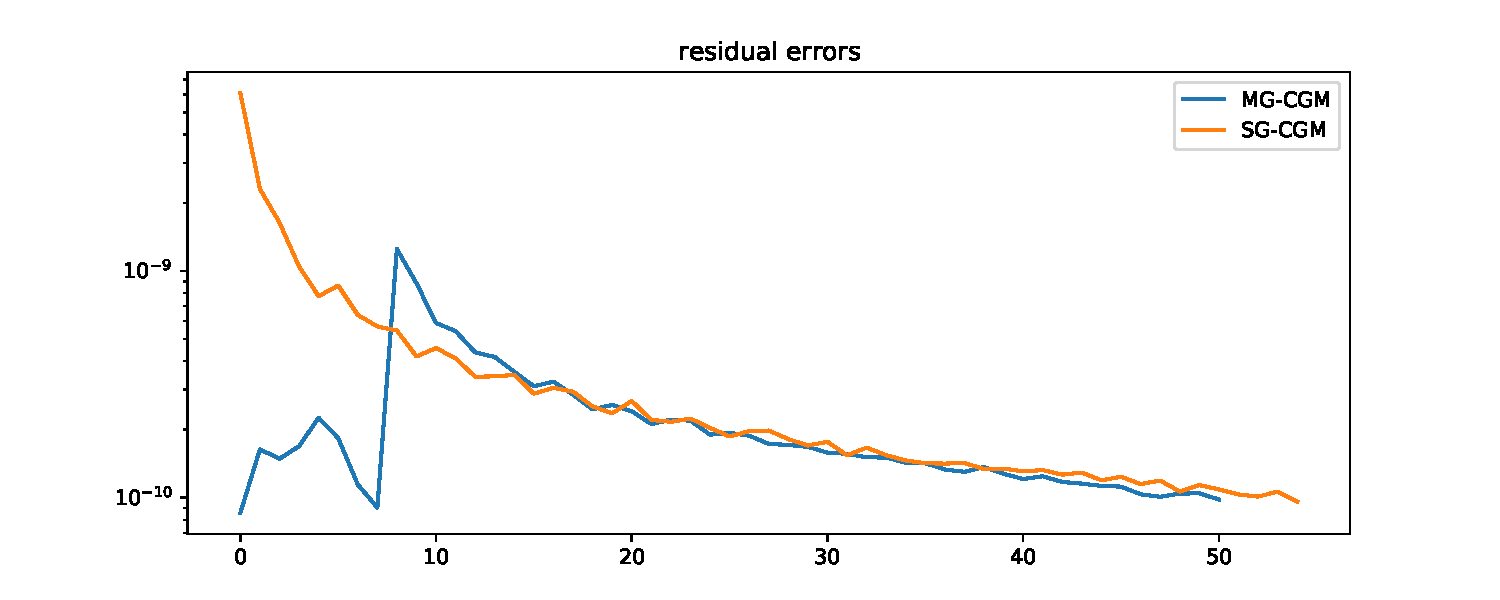
\includegraphics[width=17cm]{error.pdf}}
    \end{center}
    \small
    \qquad (a)中左图展示的是电势在求解空间中的分布情况,黑色虚线表示等势面;右图展示的是电场强度在求解空间中的分布情况,颜色的不同表示电场强度大小,箭头表示箭头根部所在的位置的电场强度矢量的方向。(b)为多重网格-共轭梯度法(MG-CGM)后迭代过程(蓝色)、直接共轭梯度法(SG-CGM)(橙色)的误差下降曲线。
    \caption{二维正弦电荷分布的数值计算结果}
    \label{F1}
\end{figure}

\subsection{点电荷分布}
设置求解区域为$S=\left\{(x,y)|-1\leq x\leq 1,-1\leq y\leq 1\right\}$的正方形区域,在两个维度上的网格精度均为$2\times 10^{-3}$,即求解区域的网格大小为$1000\times 1000$,调整多重网格等级为4,预平滑迭代次数为4,后平滑迭代求解精度为$10^{-5}$。在坐标原点放置一个$Q/\varepsilon=1/h_x h_y=0.25\times 10^{6}$的点电荷,边界条件电势为零,即(\ref{2.1a})(\ref{2.1b})式,计算其电场分布,迭代结果如图\ref{F2}(a)所示。在相同的网格和求解参数下下,另取两个绝对值相等的正负电荷组成电偶极子,分别放置在$(-0.2,0),(0.2,0)$的位置进行求解,其结果如图\ref{F2}(b)所示。

由于该问题难以给出解析解,在此处只给出定性的法分析,可以看到在正电荷处,电场方向背离电荷,在负电荷处电场方向指向电荷,在越靠近电荷的位置电场越强;在靠近边界处,电场方向均垂直于边界,符合所给定的边界条件,边界附近电场方向变化大的位置,电场强度大小较小。
\begin{figure}[ht]
    \begin{center}
        \subfigure[单点电荷]{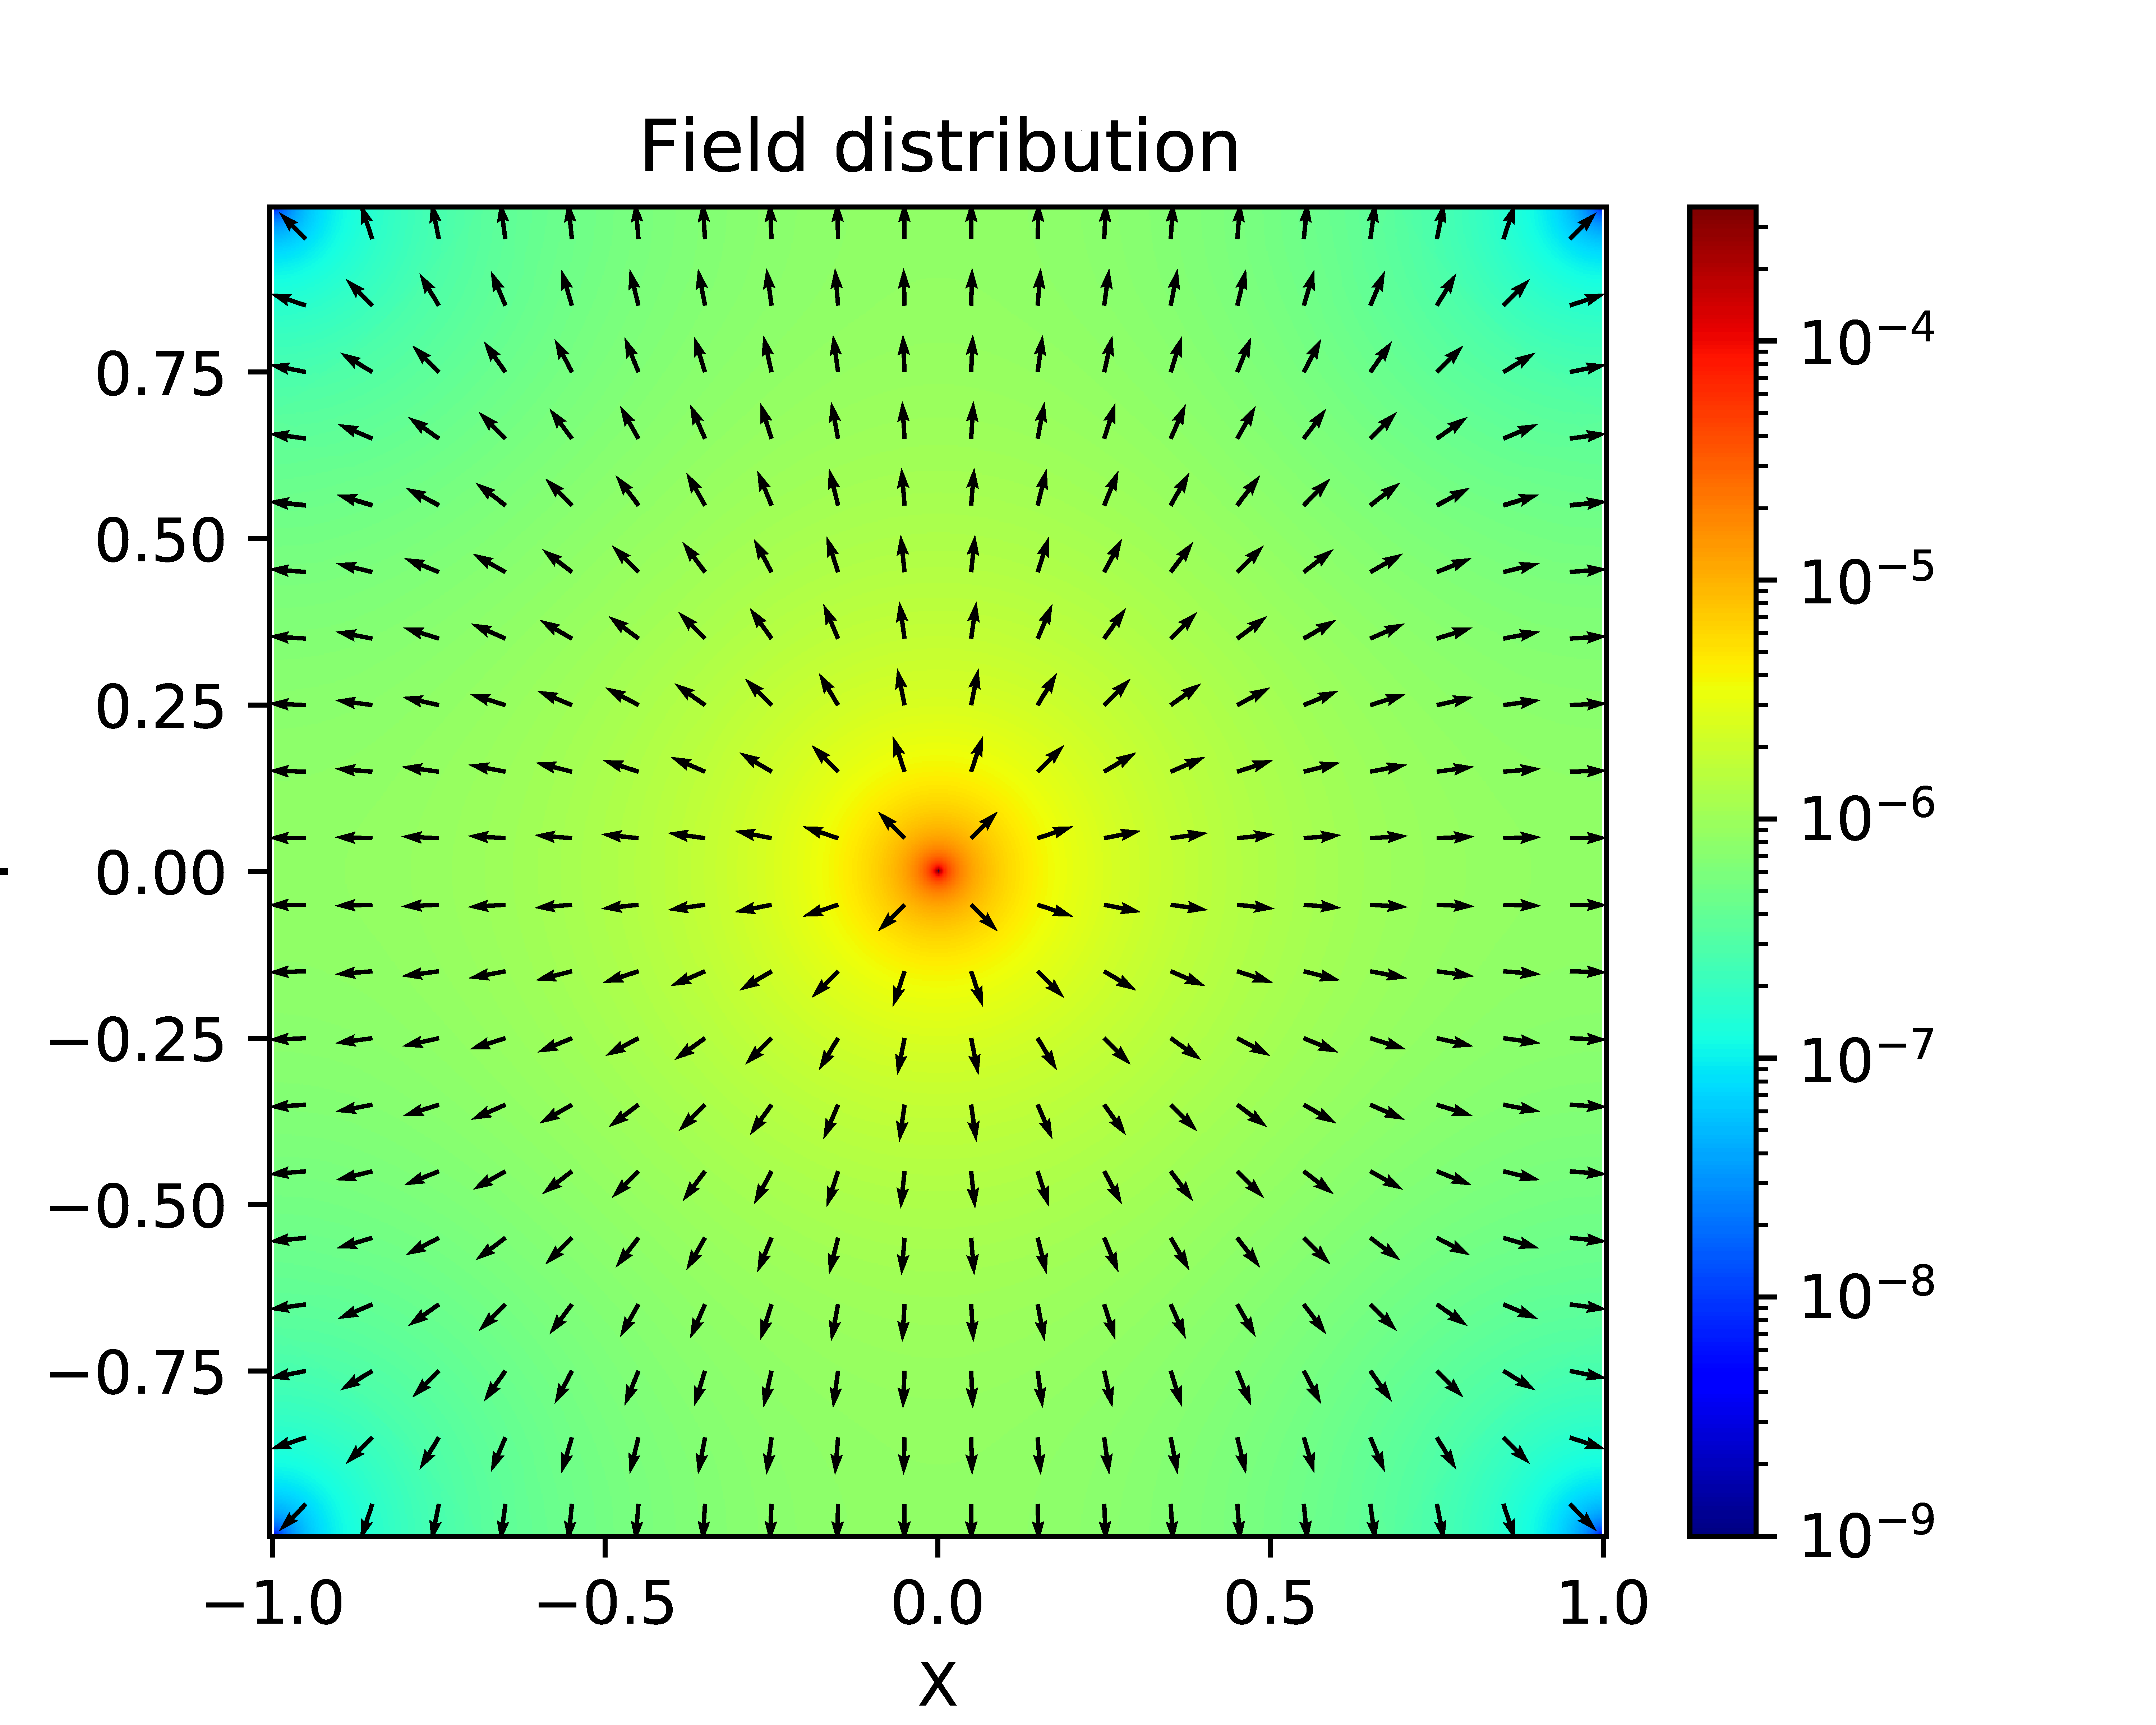
\includegraphics[width=8.2cm]{1.png}}
        \subfigure[电偶极子]{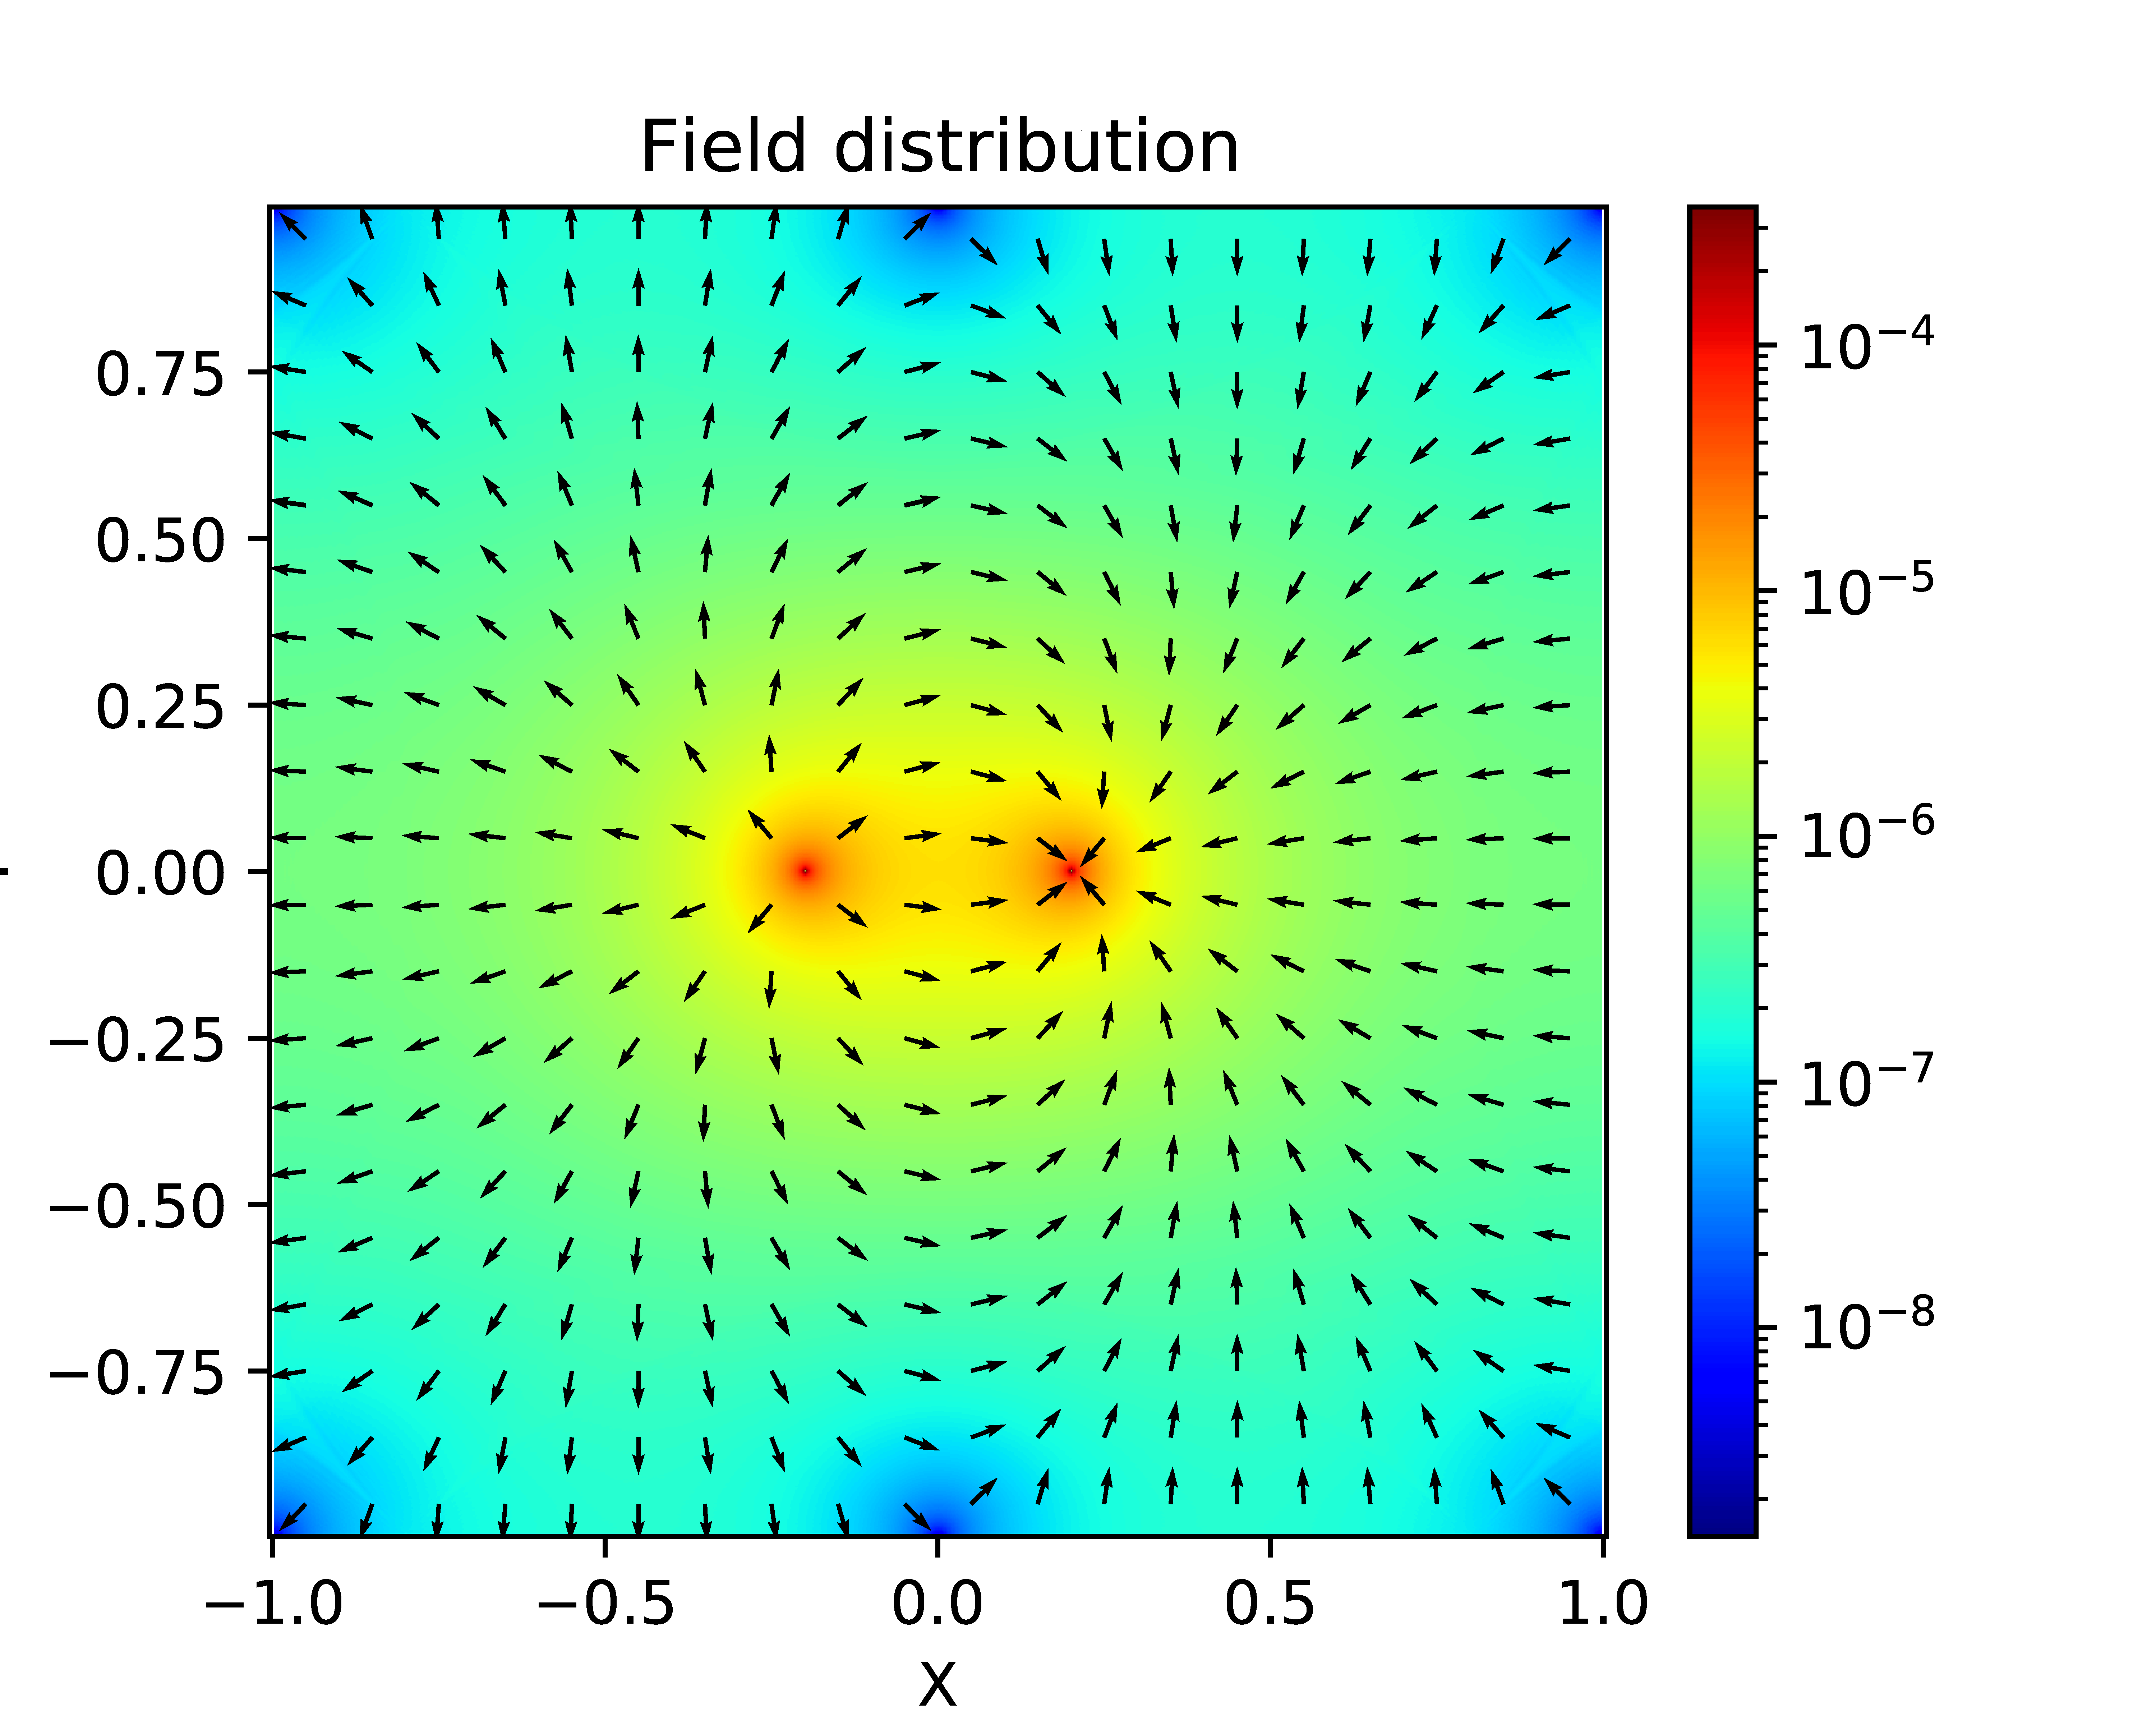
\includegraphics[width=8.2cm]{2.png}}
        \\
        \subfigure[细长带电棒]{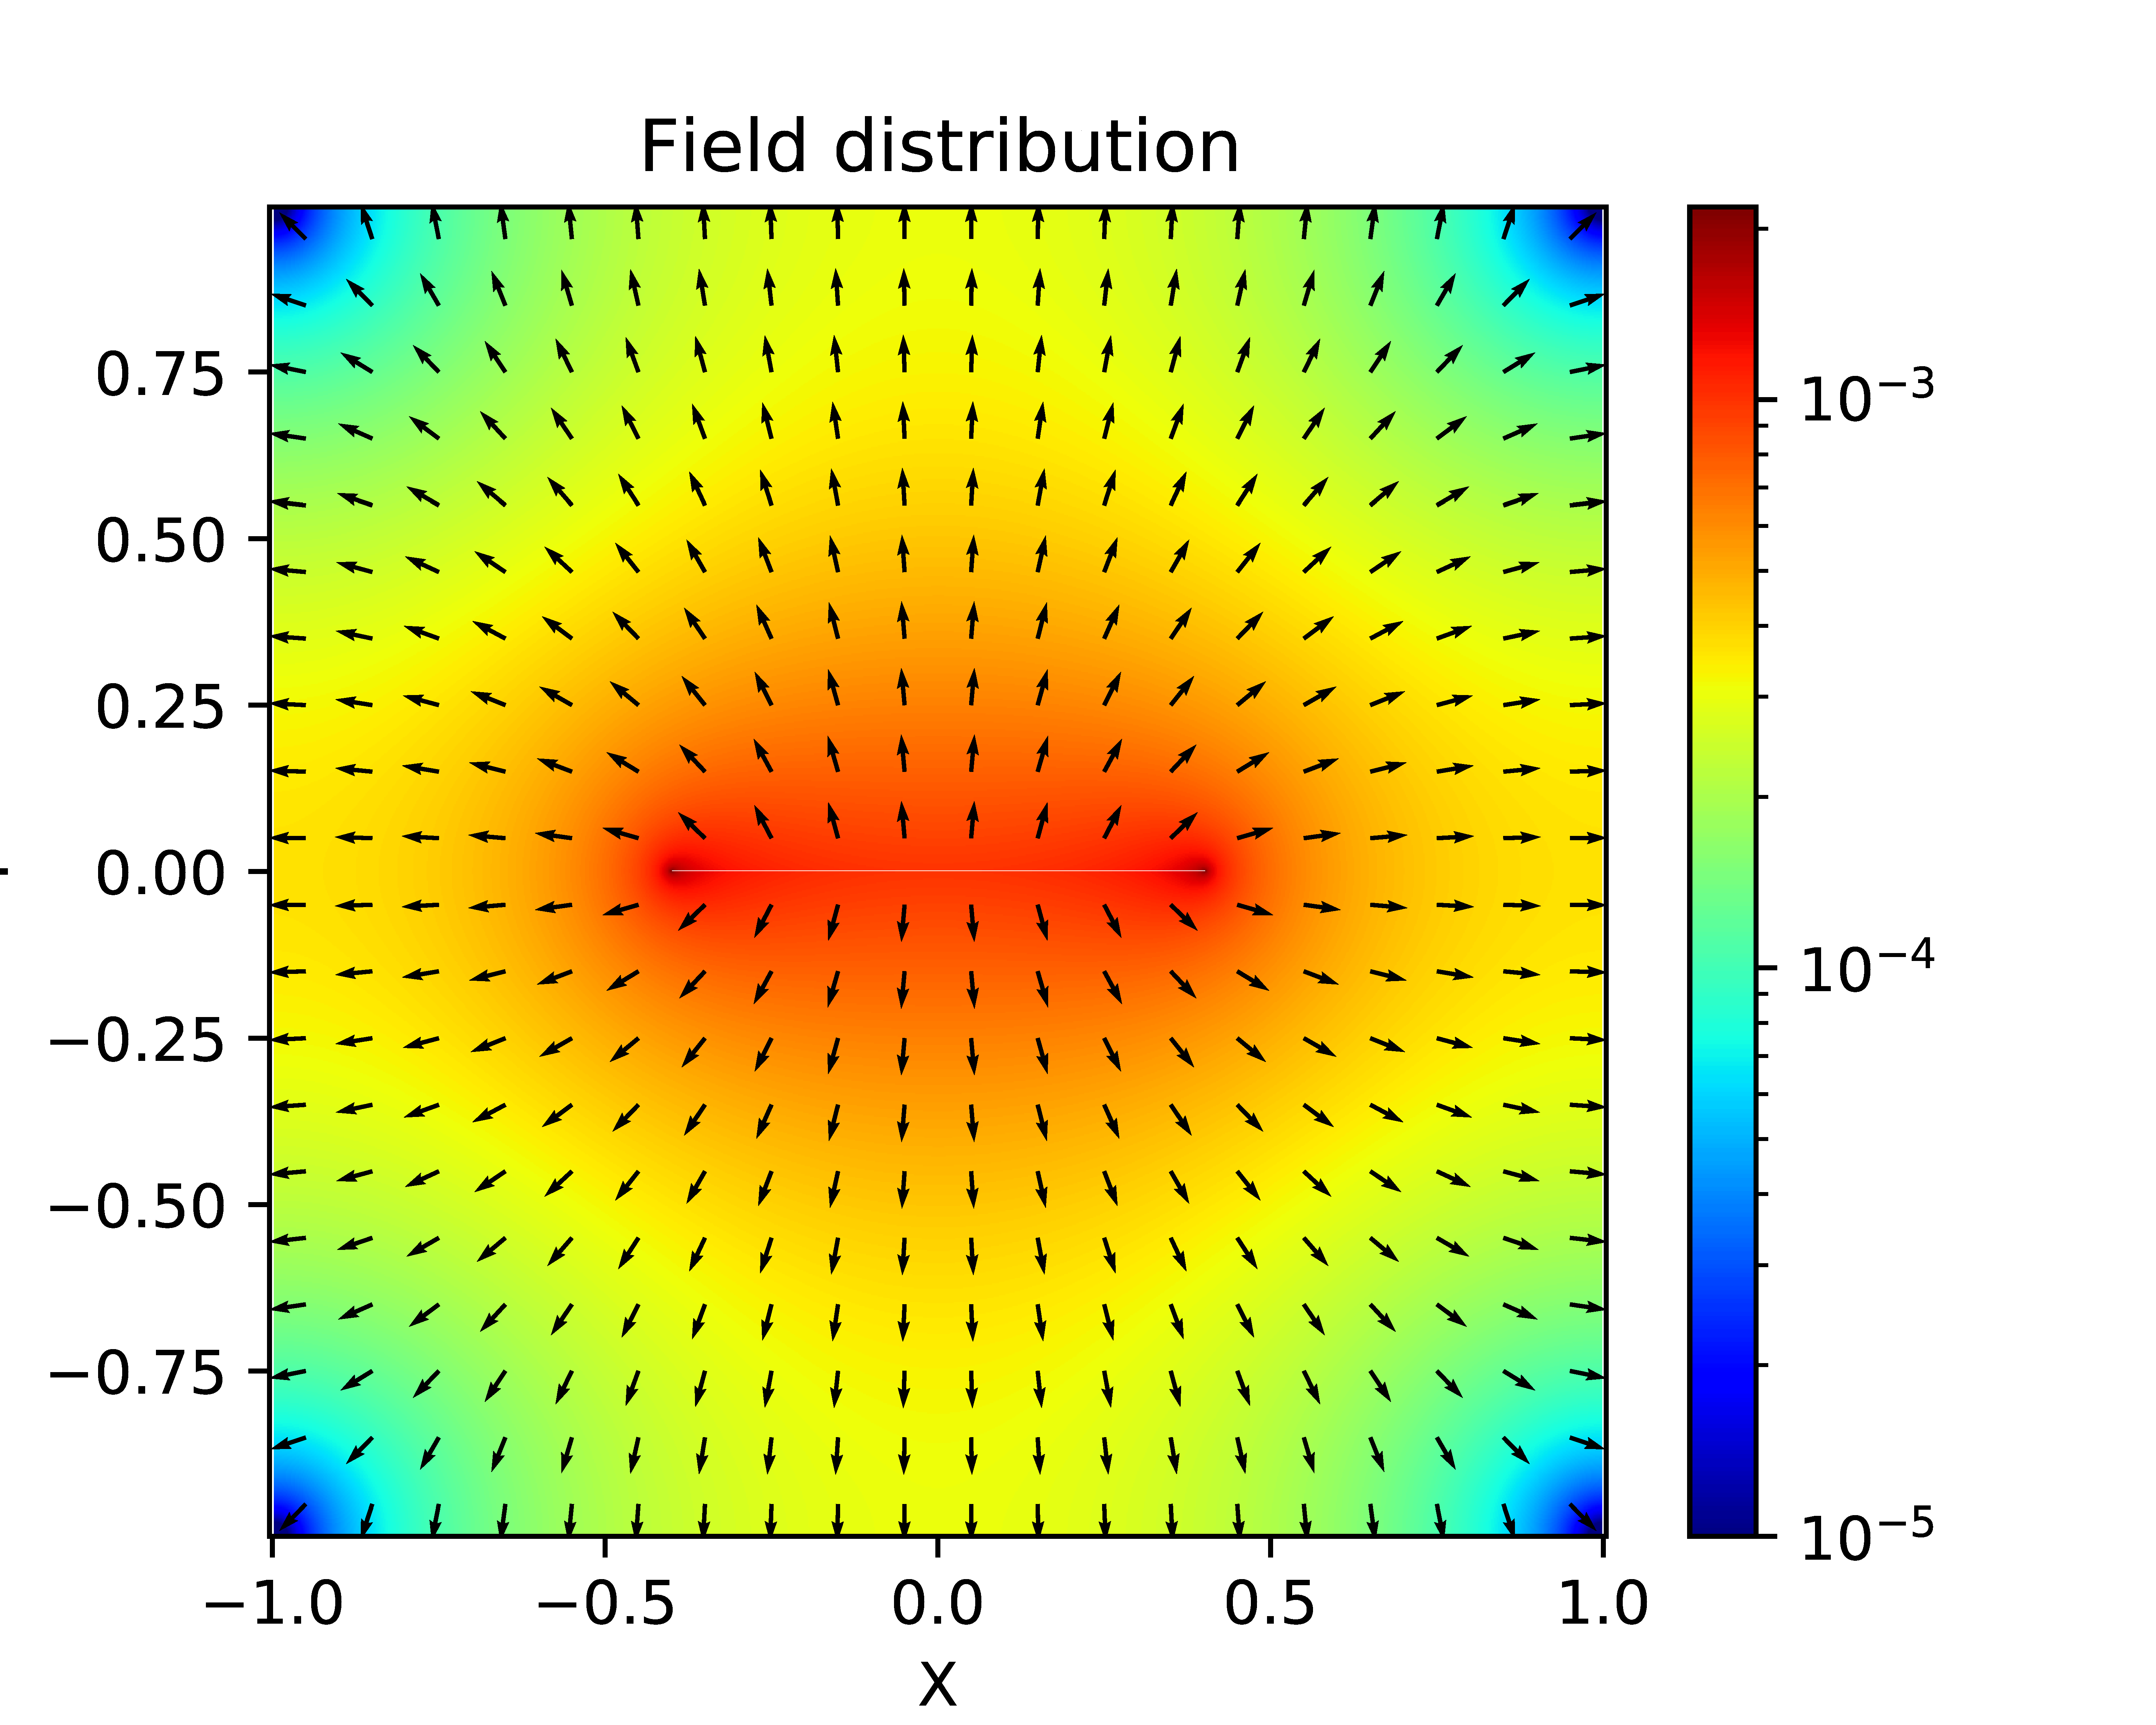
\includegraphics[width=8.2cm]{3.png}}
        \subfigure[多个带电棒]{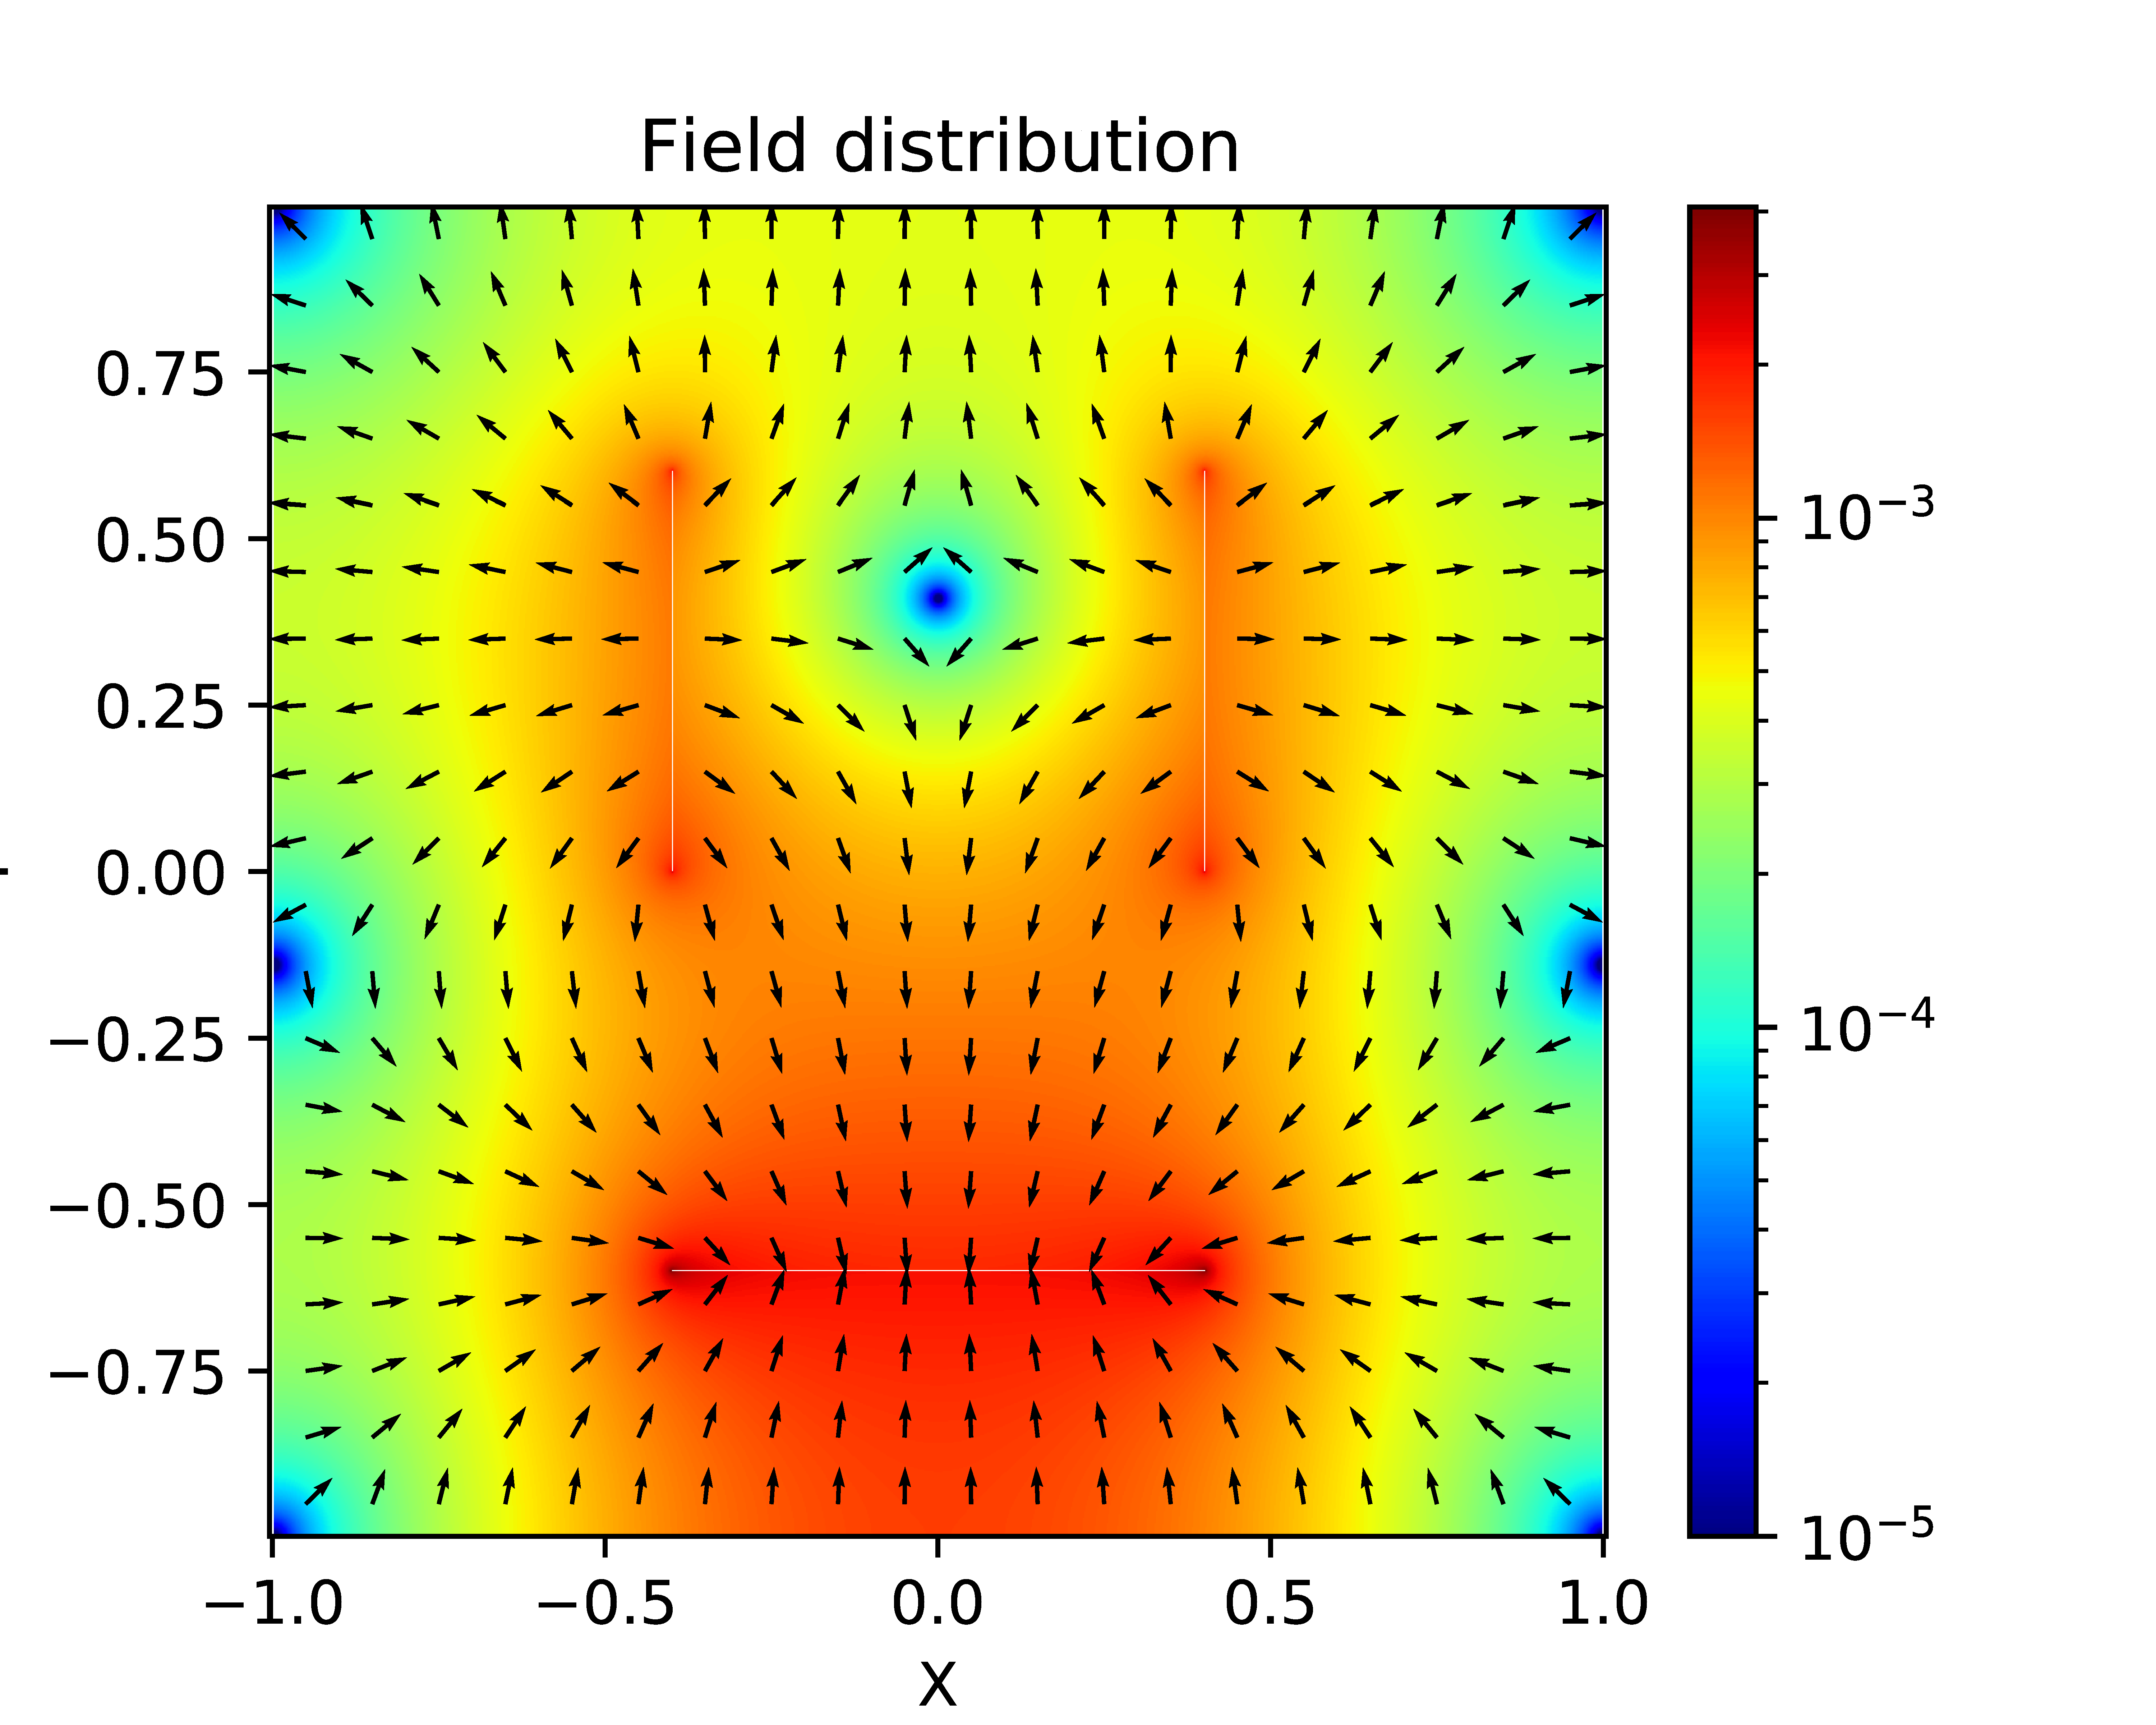
\includegraphics[width=8.2cm]{4.png}}
    \end{center}
    \caption{二维点电荷分布的数值计算电场可视化}
    \label{F2}
\end{figure}

\subsection{连续体电荷分布}
求解区域以及迭代参数与点电荷分布的数值实验设置相同,放置一根长0.8,中心位于原点的沿$x$方向的带电细棒,电荷密度为$\rho/(\varepsilon h_x h_y)=1$,边界条件设置为电势为零,即(\ref{2.1a})(\ref{2.1b})式,电场的计算结果如图\ref{F2}(3)所示。在相同的求解参数下,求解三根带电细棒在有限空间中的电场分布,计算结果如图\ref{F2}(4)所示,第一、二根细棒长0.6,沿$y$轴方向,电荷密度为$\rho/(\varepsilon h_x h_y)=1$,中心分别位于$(-0.4,0.3),(0.4,0.3)$处,第三根细棒长0.8,沿$x$轴方向,电荷密度为$\rho/(\varepsilon h_x h_y)=-2$,中心位于$(0,-0.6)$。数值实验的结果符合静静电场规律,在边界处电场方向垂直与边界,在带电帮附近,电场方向几乎垂直与细棒。

\section{讨论}

\end{document}